%Time-stamp: <sáb nov 15 15:43:04 2025 yair@asterix>
\pdfoutput=1
\documentclass{beamer}
\usepackage[utf8]{inputenc}
\usepackage{cancel}
\usepackage{xcolor}

\usepackage{hyperref}
\hypersetup{
    colorlinks=true,
    linkcolor=blue,      % links internos
    urlcolor=blue,       % URLs
    citecolor=blue,      % citações
    filecolor=blue       % links de arquivos
}

\usepackage{amsmath, amsfonts, amssymb}
\usepackage{tikz}
\usetikzlibrary{calc}

\usetheme{CambridgeUS}
\usecolortheme{beaver}

\def\Pr{\mathbb P}

\title{Embaralhamento \textit{Riffle Shuffle}}

\author[MCBM022-23]{MCBM022-23 Introdução aos Processos Estocásticos }

\date{UFABC 2025-3}

\begin{document}

\frame{\titlepage}

%------------------------------------------------------------
\begin{frame}{O que é um riffle shuffle?}
  \begin{itemize}
  \item O \textbf{riffle shuffle} é o embaralhamento típico de cassino.
  \item O baralho é dividido em duas partes e estas são intercaladas,
    \textit{preservando a ordem dentro de cada parte}.
  \end{itemize}
  
  \begin{center}
    
\includegraphics[scale=.75]{riffle1.png}
  \end{center}
\end{frame}

% ------------------------------------------------------------
\begin{frame}{Motivação}
\begin{itemize}

\item Pode ser modelado como um processo aleatório sobre as permutações
  de $n$ cartas.
\item A sequência de embaralhamentos sucessivos define naturalmente uma
  \textbf{cadeia de Markov finita}.
\end{itemize}

\vfill

\begin{block}{Pergunta central}
  Quantos embaralhamentos riffle são necessários para que o baralho
  esteja ``bem embaralhado''?
\end{block}

\vfill
\end{frame}
% ------------------------------------------------------------
\begin{frame}{Modelo}

  O baralho tem $n$ cartas, numeradas de $1$ a $n$ dispostas em
  sequência
  $$\pi=
  \begin{pmatrix}
    \pi_1,\pi_2,\dots,\pi_n
  \end{pmatrix}\quad \pi_i\in \{1,2,\dots,n\}
  $$


  um embaralhamento é uma permutação $\sigma$ de $\{1,2,\dots,n\}$
  $$ \sigma =
  \begin{pmatrix}
    \sigma(1),\sigma(2),\dots,\sigma(n-1),\sigma(n)
  \end{pmatrix}
  $$

  e $\sigma$ \textbf{age} na configuração $\pi$ embaralhando-a
  $$
    \sigma \ast \pi  =
  \begin{pmatrix}
    \pi_{\sigma(1)},
    \pi_{\sigma(2)},
    \dots,
    \pi_{\sigma(n)}
  \end{pmatrix}
  $$
  
 
\end{frame}
% ------------------------------------------------------------
\begin{frame}{Exemplo:  embaralhamento de \(    \pi = (1,2,3).  \)}

  \begin{block}{Exemplo 1: embaralhamento $\sigma = (2,1,3)$}
    \[
      \sigma \ast \pi 
      = (\pi_{\sigma(1)}, \pi_{\sigma(2)}, \pi_{\sigma(3)})
      = (\pi_2, \pi_1, \pi_3)
      = (2,1,3).
    \]
  \end{block}
  
  %\pause
  \begin{block}{Exemplo 2: embaralhamento $\sigma = (3,1,2)$}
    \[
      \sigma \ast \pi 
      = (\pi_{\sigma(1)}, \pi_{\sigma(2)}, \pi_{\sigma(3)})
      = (\pi_3, \pi_1, \pi_2)
      = (3,1,2).
    \]
  \end{block}

  %\pause
  \begin{block}{Exemplo 3: composição de embaralhamentos}
    Aplicando primeiro $\sigma_1=(2,1,3)$ e depois $\sigma_2=(3,1,2)$:
    \[
      \pi' = \sigma_1 \ast \pi = (2,1,3),
      \quad
      \pi'' = \sigma_2 \ast \pi' = (3,2,1).
    \]
    Logo:
    \(
      (1,2,3) \xrightarrow{\sigma_1=(2,1,3)} (2,1,3) 
      \xrightarrow{\sigma_2=(3,1,2)} (3,2,1).
    \)
  \end{block}

\end{frame}

% ------------------------------------------------------------
\begin{frame}{Exemplo: embaralhamento de $ \pi = (2,3,1)$ }

  \begin{block}{Exemplo 1: embaralhamento $\sigma = (2,1,3)$}
    A permutação $\sigma$ troca as duas primeiras posições:
    \[
      \sigma \ast \pi 
      = (\pi_{\sigma(1)}, \pi_{\sigma(2)}, \pi_{\sigma(3)})
      = (\pi_2, \pi_1, \pi_3)
      = (3,2,1).
    \]
  \end{block}

  %\pause
  \begin{block}{Exemplo 2: embaralhamento $\sigma = (3,1,2)$}
    A permutação $\sigma$ envia a posição $1$ para $3$, a $2$ para $1$, e a $3$ para $2$:
    \[
      \sigma \ast \pi 
      = (\pi_{\sigma(1)}, \pi_{\sigma(2)}, \pi_{\sigma(3)})
      = (\pi_3, \pi_1, \pi_2)
      = (1,2,3).
    \]
  \end{block}

  %\pause
  \begin{block}{Exemplo 3: composição de embaralhamentos}
    Aplicando primeiro $\sigma_1=(3,1,2)$ e depois $\sigma_2=(2,1,3)$:
    \[
      (2,3,1) \xrightarrow{\sigma_1=(3,1,2)} (1,2,3)
      \xrightarrow{\sigma_2=(2,1,3)} (2,1,3).
    \]
  \end{block}

\end{frame}

% ------------------------------------------------------------
\begin{frame}[c]{Espaço de estados}


  Cada configuração $( \pi_1,\pi_2,\dots,\pi_n)$ do baralho também é
  uma permutação das cartas
  $$\pi : \{1,\ldots,n\} \to \{1,\ldots,n\}, \text{ com }\pi(i)=\pi_i$$

  \vfill

  O conjunto de estados é
  \[
    \begin{aligned}
      S_n &= \{ \pi : \{1,\ldots,n\} \to \{1,\ldots,n\} \mid \pi \text{
        bijeção} \} \\ &= \left\{ \begin{pmatrix}
          \pi(1),\pi(2),\dots,\pi(n)
        \end{pmatrix}\mid 
        \pi \text{ bijeção} \right\}\\ &= \left\{ \begin{pmatrix}
          \pi_1,\pi_2,\dots,\pi_n
        \end{pmatrix}\mid 
        \pi \text{ bijeção} \right\}
    \end{aligned}
  \]

  \vfill

  O espaço de estados tem  $|S_n| = n!$ elementos.

\end{frame}
% ------------------------------------------------------------

\begin{frame}{Transições de estado}

  A transição de um estado $$\pi = (\pi_1,\pi_2,\dots,\pi_n)$$ para um
  estado $$\pi' = (\pi_1',\pi_2',\dots,\pi_n')$$ se dá pela ação
  $\ast$ de uma permutação $\sigma$
  $$
%  \begin{aligned}
    \pi' =\sigma   \ast  \pi
%    &=
%  \begin{pmatrix}
%    \pi_{\sigma(1)},
%    \pi_{\sigma(2)},
%    \dots,
%    \pi_{\sigma(n)}
%  \end{pmatrix}\\
%    &=
%  \begin{pmatrix}
%    \pi({\sigma(1)}),
%    \pi({\sigma(2)}),
%    \dots,
%    \pi({\sigma(n)})
%  \end{pmatrix}
%  \end{aligned}
  $$
  
   
  \vfill

  Essa ação é o mesmo que compor funções:
  \(\boldsymbol{\sigma \ast \pi } \equiv  \boldsymbol{ \pi \circ \sigma} \)
  
   \vfill

   Assim, o novo estado é dado pela composição das permutações
   \[\boxed{
     \pi' = \pi \circ \sigma}
   \]
   
  \vfill

  %\pause
  
  \begin{block}{\textbf{Quais permutações são permitidas agir no
        baralho?}}
\hfill    \textit{ Depende da(s) regra(s) de embaralhamento.}\hfill\ 
  \end{block}
  
\end{frame}

% ------------------------------------------------------------
% ------------------------------------------------------------
\begin{frame}{Representação binária do RF}

  \begin{block}{Riffle Shuffle}
    Um \textbf{embaralhamento riffle} é dado por uma permutação
    $\sigma$ tal que
    \[
      (\sigma(1), \sigma(2), \ldots, \sigma(n))
    \]
    é \emph{\textit{\textbf{formado por duas subsequências}
        \textbf{crescentes intercaladas}}}.
  \end{block}
  
  Ou seja, há um subconjunto $A\subseteq \{1,2,\dots,n\}$ tal que
  \begin{itemize}
  \item os elementos de $A$ aparecem em ordem crescente,
  \item os elementos de $A^{\textsc{C}}$ aparecem em ordem crescente,
  \item a sequência final $(\sigma(1),\dots,\sigma(n))$ é obtida
    intercalando essas duas subsequências.
  \end{itemize}
  
\end{frame}
% ------------------------------------------------------------
\begin{frame}{Representação binária do RF}
  \begin{itemize}
  \item Cada carta pode vir da \textbf{mão esquerda}
    ($\mathrm{\mathbf{0}}$) ou da \textbf{mão direita}
    ($\mathtt{\mathbf{1}}$).
  \item Assim, cada embaralhamento riffle~pode ser representado por uma
    sequência binária de comprimento $n$.
  \end{itemize}
  
  
  \only<1>{
    \begin{exampleblock}{Exemplo para $n=5$}
      \[
        01101 \;\Rightarrow\; \text{1ª e 4ª carta de \textbf{0}, 2ª, 3ª
          e 4ª de \textbf{1} .}
      \]
    \end{exampleblock}
    
    \[
      \Rightarrow \text{Existem } 2^n \text{ sequências possíveis.}
    \]}
  
  
  \only<2>{
    
    \begin{center}
      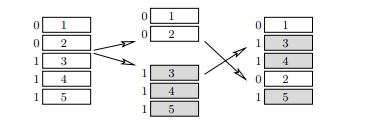
\includegraphics[scale=.55]{embaralhada.png}
    \end{center}
    
  }

\end{frame}
% ------------------------------------------------------------
\begin{frame}{Exemplo para $n=3$}
 
Cartas: $(1,2,3)$

\begin{center}
\begin{tabular}{c||c|l}
\textbf{Corte} & \textbf{Padrão binário} & \textbf{Permutação} \\
 \hline
$123|$ & 000 & $(1,2,3)$ \\
\hline%\pause
$12|3$ & 001 & $(1,2,3)$ \\ 
\hline
$12|3$ & 010 & $(1,3,2)$ \\
\hline
$12|3$ & 100 & $(3,1,2)$ \\
\hline%\pause
$1|23$ & 011 & $(1,2,3)$ \\
\hline
$1|23$ & 101 & $(2,1,3)$ \\
\hline
$1|23$ & 110 & $(2,3,1)$ \\
\hline%\pause
$|123$ & 111 & $(1,2,3)$ \\
\end{tabular}
\end{center}

\vfill

\phantom{São 8 configurações com 5 delas  distintas.}

\vfill
\end{frame}
% ------------------------------------------------------------
\begin{frame}{Exemplo para $n=3$}
 
Cartas: $(1,2,3)$

\begin{center}
\begin{tabular}{c||c|l}
\textbf{Corte} & \textbf{Padrão binário} & \textbf{Permutação} \\
 \hline
$123|$ & 000 & $(1,2,3)$  \\
\hline
$12|3$ & 001 & \cancel{$(1,2,3)$} \\ 
\hline
$12|3$ & 010 & $(1,3,2)$  \\
\hline
$12|3$ & 100 & $(3,1,2)$   \\
\hline
$1|23$ & 011 & \cancel{$(1,2,3)$ } \\
\hline
$1|23$ & 101 & $(2,1,3)$ \\
\hline
$1|23$ & 110 & $(2,3,1)$  \\
\hline
$|123$ & 111 & \cancel{$(1,2,3)$ }\\
\end{tabular}
\end{center}

\vfill

\emph{São 8 configurações com 5 delas  distintas.}

\vfill

\end{frame}
% ------------------------------------------------------------
\begin{frame}{Quando duas sequências geram o mesmo shuffle?}
  \begin{itemize}
  \item Nem todas as $2^n$ sequências produzem permutações distintas.
  \item Se todas as cartas forem para o mesmo lado:
    \[
      000\ldots0 \quad \text{ou} \quad 111\ldots1,
    \]
    então o baralho não se altera (perm. identidade).
  \item Ou com intercalação trivial de $\mathrm{\mathbf{0}} = [1,\dots,k]$ e
    $\mathrm{\mathbf{1}}=[k+1,\dots,n]$ para $k=1,2,\dots,n-1$.
  \end{itemize}
  %\pause
  \[
    \Rightarrow \text{Devemos subtrair esses } n \text{ casos degenerados.}
  \]
  \[
    \boxed{
      \text{Número de riffle shuffles distintos} = 2^n - n
    }
  \]
  
\end{frame}
% ------------------------------------------------------------
\begin{frame}{Transições}

  Cada passo da cadeia corresponde a um \emph{riffle shuffle}
  aleatório.

  \bigskip
  
  Há três descrições \textbf{equivalentes} para a distribuição de
  transição $\mathrm{Rif}(\sigma)$:

\end{frame}
% ------------------------------------------------------------
\begin{frame}{Descrição combinatória}

  \[
    \mathrm{Rif}(\sigma)
    =
    \begin{cases}
      \dfrac{n+1}{2^n}, & \text{se } \sigma = \mathrm{id},\\[10pt]
      \dfrac{1}{2^n}, & \text{se } \sigma \text{ é formada por duas subsequências crescentes},\\[10pt]
      0, & \text{caso contrário}.
    \end{cases}
  \]
\end{frame}
% ------------------------------------------------------------
\begin{frame}{Descrição combinatória $n=3$}
  \begin{center}
    \begin{tabular}{c|c|c}
      \textbf{Corte} & $\sigma$ & $\mathrm{Rif}(\sigma)$ \\
      \hline
      $123|$, $12|3$, $1|23$, $|123$ & $(1,2,3)$ & $\tfrac{4}{8}$ \\[.5em]
      $12|3$ & $(1,3,2)$ & $\tfrac{1}{8}$ \\[.5em]
      $12|3$ & $(3,1,2)$ & $\tfrac{1}{8}$ \\[.5em]
      $1|23$ & $(2,1,3)$ & $\tfrac{1}{8}$ \\[.5em]
      $1|23$ & $(2,3,1)$ & $\tfrac{1}{8}$
    \end{tabular}
  \end{center}
\end{frame}
% ------------------------------------------------------------
\begin{frame}{Descrição probabilística (modelo físico)}

  Corta-se o baralho em duas partes: uma com $t$ e a outra com $n-t$
  cartas. O corte ocorre no ponto $t$ com probabilidade
  \[
    \frac{\binom{n}{t}}{2^n}.
  \]
  
  As duas metades são então entrelaçadas: quando há $r$ cartas na mão
  direita e $\ell$ na esquerda, a próxima carta vem da direita com
  probabilidade $\dfrac{r}{r+\ell}$ e da esquerda com probabilidade
  $\dfrac{\ell}{r+\ell}$.

\end{frame}
% ------------------------------------------------------------
\begin{frame}{Descrição probabilística (modelo físico) $n=3$}
  \begin{table}[h!]
    \centering
    \begin{tabular}{c|c|c|l}
      $t$  & corte & probabilidade do corte & resultados possíveis \\ \hline
      0 & $|123$ & $\frac{1}{8}$ & (1,2,3) \\[.5em]
      1 & $1|23$ & $\tfrac{3}{8}$ & (1,2,3), (2,1,3), (2,3,1) \\[.5em]
      2 & $12|3$ & $\tfrac{3}{8}$ & (1,2,3), (1,3,2), (3,1,2) \\[.5em]
      3 & $123|$ & $\tfrac{1}{8}$ & (1,2,3) 
    \end{tabular}
  \end{table}
  
\end{frame}
% ------------------------------------------------------------
\begin{frame}{Descrição inversa}

  Atribui-se a cada carta um rótulo $0$ ou $1$, independentemente e com
  probabilidade $1/2$ cada.

  Move-se todas as cartas com rótulo $0$ para o topo, preservando a
  ordem relativa dentro de cada grupo.

  Essa operação define a permutação inversa de um \emph{riffle
    shuffle}.


  \begin{center}
    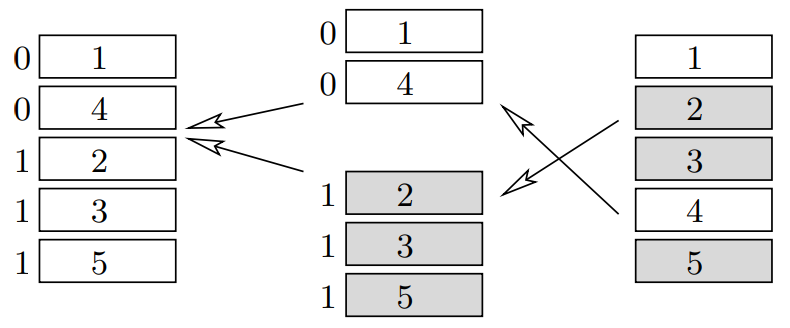
\includegraphics[scale=.25]{inversa.png}
  \end{center}
  
\end{frame}
% ------------------------------------------------------------
\begin{frame}{ Descrição inversa para \(n=3\)}

  \begin{center}
    \begin{tabular}{c|c|c}
      \textbf{Rótulos} & \textbf{Resultado (nova ordem)} & \textbf{Permutação inversa $\sigma^{-1}$}\\
      \hline
      (0,0,0) & (1,2,3) & (1,2,3) \\[.3em]
      (0,0,1) & (1,2,3) & (1,2,3) \\[.3em]
      (0,1,0) & (1,3,2) & (1,3,2) \\[.3em]
      (1,0,0) & (2,3,1) & (2,3,1) \\[.3em]
      (0,1,1) & (1,2,3) & (1,2,3) \\[.3em]
      (1,0,1) & (2,1,3) & (2,1,3) \\[.3em]
      (1,1,0) & (3,1,2) & (3,1,2) \\[.3em]
      (1,1,1) & (1,2,3) & (1,2,3)
    \end{tabular}
  \end{center}

\end{frame}
% ------------------------------------------------------------
\begin{frame}{A cadeia de Markov do R.S.}

  A cadeia de Markov $(X_n)_{n\ge0}$ do embaralhamento Riffle:

  \begin{itemize}\itemsep=.3cm
  \item $S_n= \{ \pi\colon \pi \text{ permutação de  }  1,2,\dots,n\}$
  \item $X_0 = \mathrm{id}$;
  \item $X_{n+1} = X_n\circ \sigma$ com probabilidade $\mathrm{Rif}(\sigma)$.
  \end{itemize}

  \vfill


  A matriz de transição $P = (p_{\pi,\pi'})$ é dada por

  \[
    p_{\pi,\pi'} =  \mathrm{Rif}(\pi^{-1}\circ\pi') .
  \]
  
  pois se $\pi' = \pi\circ\sigma$ então $\sigma = \pi^{-1}\circ\pi'$.
  
  
\end{frame}
% ------------------------------------------------------------
\begin{frame}{Exemplo $n=3$}{Matriz de transições em termos de $\sigma = \pi^{-1} \circ \pi'$}

 \[
    E_{\pi,\pi'} = \sigma
  \]

  \[
    \begin{array}{c|cccccc}
 $E$     & (1,2,3) & (1,3,2) & (2,1,3) & (2,3,1) & (3,1,2) & (3,2,1) \\ \hline
      (1,2,3) & \textcolor{blue}{(1,2,3)} & (1,3,2) & (2,1,3) & (2,3,1) & (3,1,2) & \textcolor{red}{(3,2,1)} \\[6pt]
      (1,3,2) & (1,3,2) & \textcolor{blue}{(1,2,3)} & (2,3,1) & \textcolor{red}{(3,2,1)} & (2,1,3) & (2,3,1) \\[6pt]
      (2,1,3) & (2,1,3) & (2,3,1) & \textcolor{blue}{(1,2,3)} & (1,3,2) & \textcolor{red}{(3,2,1)} & (3,1,2) \\[6pt]
      (2,3,1) & (3,1,2) &  \textcolor{red}{(3,2,1)} & (1,3,2) & \textcolor{blue}{(1,2,3)} & (2,3,1) & (2,1,3) \\[6pt]
      (3,1,2) & (2,3,1) & (2,1,3) & \textcolor{red}{(3,2,1)} & (3,2,1) & \textcolor{blue}{(1,2,3)} & (1,3,2) \\[6pt]
      (3,2,1) &  \textcolor{red}{(3,2,1)} & (3,1,2) & (2,3,1) & (2,1,3) & (1,3,2) & \textcolor{blue}{(1,2,3)}      
  \end{array}
\]


\end{frame}
% ------------------------------------------------------------
\begin{frame}{Matriz de transição \(P\) para \(n=3\)}

  \[
\begin{array}{c|cccccc}
 & 123 & 132 & 213 & 231 & 312 & 321 \\ \hline 
123 & 1/2 & 1/8 & 1/8 & 1/8 & 1/8 & 0 \\[15pt]
132 & 1/8 & 1/2 & 1/8 & 0   & 1/8 & 1/8 \\[15pt]
213 & 1/8 & 1/8 & 1/2 & 1/8 & 0   & 1/8 \\[15pt]
231 & 1/8 & 0   & 1/8 & 1/2 & 1/8 & 1/8 \\[15pt]
312 & 1/8 & 1/8 & 0   & 1/8 & 1/2 & 1/8 \\[15pt]
321 & 0   & 1/8 & 1/8 & 1/8 & 1/8 & 1/2
\end{array}
\]

\end{frame}
% ------------------------------------------------------------
\begin{frame}{A matriz é duplamente estocástica} 

  De fato, $P$ é simétrica:

  \vfill

  \begin{enumerate}
  \item $\sigma=\mathrm{id}$ se e só se  $\sigma^{-1}=\mathrm{id}$.
  \item $\sigma$ é formada por duas subsequências crescentes se e só se
    $\sigma^{-1}$ é formada por duas subsequências crescentes.
  \end{enumerate}
  
  
  \vfill
  
  Portanto, $\mathrm{Rif}(\sigma)= \mathrm{Rif}(\sigma^{-1})$.
  
  \vfill

  Se $\pi' = \pi\circ\sigma$ então $\pi=\pi'\circ \sigma^{-1}$, logo

  $$
  p_{\pi,\pi'} = \mathrm{Rif}(\sigma) = \mathrm{Rif}(\sigma^{-1}) = p_{\pi',\pi} .
  $$

  \vfill
  
  $P$ é simétrica, portanto duplamente estocástica se estocástica:
   \end{frame}
% ------------------------------------------------------------
\begin{frame}{A matriz é duplamente estocástica} 
  Soma de linha:
  \[
    \sum_{\pi' \in S_n} p_{\pi, \pi'}
    = \sum_{\pi' \in S_n} \mathrm{Rif}(\pi^{-1} \circ \pi')
    = \sum_{\sigma \in S_n} \mathrm{Rif}(\sigma) = 1,
  \]
  pois a função \(\pi' \mapsto \pi^{-1} \circ \pi'\) é uma bijeção em
  \(S_n\) e \(\mathrm{Rif}\) é uma distribuição de probabilidade sobre
  \(S_n\). \textbf{É estocástica}.
  
  \vfill
  
  Agora, só conferindo a soma das colunas 
  \[
    \sum_{\pi \in S_n} p_{\pi, \pi'} = \sum_{\pi \in S_n}
    \mathrm{Rif}(\pi^{-1} \circ \pi')= \sum_{\sigma \in S_n}
    \mathrm{Rif}(\sigma) = 1
  \]
  
  Substituindo \(\sigma = \pi^{-1} \circ \pi'\), o que implica
  \(\pi = \pi' \circ \sigma^{-1}\).  Mais uma vez, a transformação
  \(\pi \mapsto \sigma\) é bijetora.
\end{frame}
% ------------------------------------------------------------
\begin{frame}{Estrutura da cadeia}

  \vfill
  
  A cadeia é irredutível (qualquer permutação pode ser atingida após
  número finito de embaralhamentos).

  \vfill
  
  A cadeia é aperiódica: $p_{\pi,\pi}> 0$ pois $\sigma=\mathrm{id}$ é
  embaralhamento.

  \vfill
  
  A distribuição invariante é a distribuição uniforme
  \[
    U(\sigma) = \frac{1}{n!}
  \]
  pois é coluna-estocástica.
\end{frame}
% ------------------------------------------------------------
\begin{frame}[fragile]{Dinâmica markoviana}{Distribuição nos estados}

  \vfill

  Distribuição inicial:
  \begin{center}  
    $X_0\sim\mathrm{Rif}^{(0)} = \left( \delta_{\mathrm{id},\pi}
    \right)_{\pi\in S_n  }$ vetor estocástico concentrado em
    $\pi=\mathrm{id}$.
  \end{center}

  \vfill

  Distribuição $k\ge1$ passos:

$$\mathrm{Rif}^{(k)} = \mathrm{Rif}^{(k-1)} \,\cdot\, P$$
  
  \vfill

  \emph{A cadeia é ergódica}:
  $$
  \mathrm{Rif}^{(k)}
  \xrightarrow[]{k\to \infty} U
  $$
  
  \vfill%\pause

  \begin{block}{Pergunta central}
    Quantos embaralhamentos riffle são necessários para que o baralho
    esteja ``bem embaralhado''?
  \end{block}
  
  \vfill
  

\end{frame}
% ------------------------------------------------------------

\begin{frame}{``bem embaralhado'' --- Distância de variação total}
  
  \textbf{Definição.}  Sejam $P$ e $Q$ duas distribuições de
  probabilidade sobre um mesmo espaço finito $\Omega$.  A
  \emph{distância de variação total} entre $P$ e $Q$ é:
  \[
    \|P - Q\|_{{\textsf{TV}}}
    \;\; = \;\;  \frac{1}{2} \sum_{x \in \Omega} |P(x) - Q(x)|
    \;\;  = \;\;  \max_{A \subseteq \Omega} |P(A) - Q(A)|.
  \]
  
  %\pause
  \textbf{Interpretação:}
  \begin{itemize}
  \item Mede o maior desvio possível entre as probabilidades atribuídas
    por $P$ e $Q$ a um mesmo evento $A$.
  \item Mede a fração da
    probabilidade total que teria de ser ``movida'' para transformar
    $P$ em $Q$.
    
    %\pause
    
  \item $\mathrm{Rif}^{(k)}$ distribuição após $k$ embaralhamentos, $U$
    dist.~uniforme
    \[
      \| \mathrm{Rif}^{(k)} - U\|_{{\textsf{TV}}}
      = 0{,}1
      \;\;\text{ significa que o baralho está 90\% misturado.}
    \]  
  \end{itemize}
\end{frame}
% ------------------------------------------------------------
\begin{frame}{Por que as duas expressões são iguais?}
 
  \[
     \frac{1}{2} \sum_{x \in \Omega} |P(x) - Q(x)|
    = \max_{A \subseteq \Omega} |P(A) - Q(A)|.
  \]
  
  %\pause
  \begin{itemize}\itemsep=.4cm
    
  \item Conjunto ótimo $A^\ast$ é aquele onde $P(x) > Q(x)$ sse 
    $x\in A^\ast$.
  
  \item \( P(A) - Q(A) = \sum_{x \in A} [P(x) - Q(x)].  \)
    
  \item
    \( P(A^\ast) - Q(A^\ast) = \sum_{x : P(x) > Q(x)} [P(x) - Q(x)].
    \)
      
  \item
    $\displaystyle\sum_x [P(x) - Q(x)] = 0 \Rightarrow \sum_{x \in
      A^\ast} |P(x) - Q(x)| = \sum_{x \notin A^\ast} |P(x) - Q(x)| $
    \[
      \sum_{x : P(x) > Q(x)} [P(x) - Q(x)]
      = \tfrac{1}{2} \sum_{x \in \Omega} |P(x) - Q(x)|.
    \]
  \end{itemize}
  
  
\end{frame}

% ------------------------------------------------------------

\begin{frame}{Distância de variação total — ideia visual (discreta)}


{
  \begin{center}
    \includegraphics<1>[scale=.5]{tv1.png}
    \includegraphics<2>[scale=.5]{tv2.png}
  \end{center}
}
  
\end{frame}

% ------------------------------------------------------------
\begin{frame}{Distância de variação total — C.M.}

  \begin{block}{Definição}
  Seja \((X_n)_n\) uma cadeia de Markov ergódica com matriz de
  transição $P$ e distribuição limite \(\pi\).  A \textbf{distância de
    variação total} no tempo \(k\) é
  
  \[
    \begin{aligned}
      d(k) &= \max_{i \in {S}} \; \max_{A \subseteq {S}} \bigl|
      \Pr(X_k \in A \mid X_0 = i) - \pi(A) \bigr|\\[1em]
      &= \max_{i \in {S}} \; \frac12 \sum_{j\in S} \bigl|
      p_{i,j}^{(k)} - \pi_j  \bigr|\\
    \end{aligned}
  \]
\end{block}



A medida de distância assume valores entre \(0\) e \(1\).  Se
\(d(k) = 0\), então a cadeia está em estacionariedade no tempo \(k\).
Com o passar do tempo, \(d(k) \to 0\) quando \(k \to \infty\).
  
\end{frame}
% ------------------------------------------------------------

\begin{frame}{Tempo de mistura}


%\pause
O \textbf{tempo de mistura} $t_{\text{mix}}(\varepsilon)$ é o menor $k$ tal que $d(k) \le \varepsilon$.

%\pause
\begin{exampleblock}{\href{https://www.stat.berkeley.edu/~aldous/157/Papers/bayer_diaconis.pdf}{[Resultado de Bayer e Diaconis (1992)}]:}
Para o modelo de riffle shuffle:
\[
t_{\text{mix}} \approx \frac{3}{2}\log_2 n.
\]
Em particular, para um baralho de $n=52$ cartas:
\[
t_{\text{mix}} \approx 7 \text{ embaralhamentos.}
\]
\end{exampleblock}
\end{frame}

% ------------------------------------------------------------
\begin{frame}[c]{Teorema principal}

  \vfill
  
  Vamos demonstrar menos:

  \vfill
  
  \begin{block}{}
    \[
      \boxed{
        \|{\rm Rif}^{(k)} - U\|_{\textsf{TV}}
          \le 1 - \prod_{i=1}^{n-1}\Big(1 - \frac{i}{2^k}\Big)
        }
      \]
    \end{block}

  \vfill
  
    O que permite concluir que $k=12$ é suficiente.
    
  \vfill
  
  
\end{frame}
%------------------------------------------------------------
\begin{frame}{Regra de parada fortemente uniforme}

  \textbf{Ideia:} queremos um tempo de parada $T$ tal que, no instante
  $T$, a permutação do baralho seja \emph{exatamente uniforme}.
  
  \begin{block}{Definição}
    Um tempo de parada $T$ é \textbf{fortemente uniforme} se
    \[
      \Pr[X_k = \pi \mid T = k] = \tfrac{1}{n!}, \quad
      \forall\,\pi \in S_n .
    \]
    Em particular $X_T$ é independente de $T$ e é uniformemente
    distribuído.
  \end{block}
  
\end{frame}

% ------------------------------------------------------------
\begin{frame}{Lema: controle da mistura por tempo de parada forte}
  {Tempos fortemente estacionários e Distância de variação total}

  
  \textbf{Lema.} Seja \(T\) um tempo fortemente estacionário para uma
  cadeia de Markov ergódica. Para \(k > 0\),
  \[
    d(k) \le \Pr(T > k).
  \]
  
  \textbf{Corolário.}  \textit{Sejam $Q$, $Q^{(k)}$ e $U$ distribuições
    de probabilidade em $S_n$; $Q$ define um processo de
    embaralhamento, $Q^{(k)}$ a distribuição obtida aplicando o
    processo $k$ vezes e $U$ a distribuição uniforme. Se o processo
    admite tempo de parada $T$ para uma \textrm{regra de parada
      fortemente uniforme}, então para todo $k \ge 0$,}
  \[
    \| Q^{(k)} - U \|_{{\textsf{TV}}} \;\le\; \Pr[T > k].
  \]
  
 
\end{frame}
% ------------------------------------------------------------
\begin{frame}{Demonstração detalhada}

 

  Para $S \subseteq S_n$, seja
  \[
    Q^{(k)}(S) = \Pr(X_k \in S).
  \]
  
  %\pause
  
  Como $T$ é o tempo de parada forte,
  temos para todo $j \le k$
  %
  $$\Pr(X_k \in S,\, T = j) =\Pr(X_k \in S)\Pr(T = j) = U(S)\Pr(T = j)$$
  
  %\pause
  
  \[
    \begin{aligned}
      Q^{(k)}(S) 
      &= \Pr(X_k \in S,\, T>k)
      + \sum_{j: j \le k} \Pr(X_k \in S,\, T=j)  \\[0.5em]%\pause
      &=  \Pr(X_k \in S \mid T>k) \Pr(T>k)
      + U(S)\!\sum_{j: j \le k} \Pr(T=j)\\[0.5em]
      &= \Pr(X_k \in S \mid T>k)\Pr(T>k)
      + U(S)(1-\Pr(T>k)) 
    \end{aligned}
  \]
  
\end{frame}

% ------------------------------------------------------------
\begin{frame}{Demonstração detalhada}

   \[
     Q^{(k)}(S)= \Pr(X_k \in S \mid T>k)\Pr(T>k) + U(S)(1-\Pr(T>k))
   \]
   
   
   Portanto,
   \[
     Q^{(k)}(S) - U(S) = \bigl(\Pr[X_k \in S \mid T>k] -
     U(S)\bigr)\,\Pr[T>k].
   \]
   
   %\pause
   Como o termo entre parênteses tem valor absoluto $\le 1$,
   \[
     \vert \,Q^{(k)}(S) - U(S)\,\vert  \le \Pr[T > k].
   \]
   Tomando o máximo em $S\subseteq S_n$,
   \[
     \boxed{\|Q^{(k)} - U\|_{{\textsf{TV}}} \le \Pr[T>k].}
   \]\qed
 \end{frame}
 
%------------------------------------------------------------
\begin{frame}
{A regra de parada}
{Modelo do riffle shuffle invertido}

  \begin{itemize}
  \item A cada carta atribuímos independentemente um rótulo binário
    $b_i \in \{0,1\}$.
  \item As cartas com $b_i=0$ vão para o topo,\textit{ mantendo a ordem
      relativa} dentro de cada grupo.
  \item Repetindo o procedimento $k$ vezes equivale a dar a cada carta
    um rótulo de $k$ bits, isto é, um número em $\{0,1,\dots,2^k-1\}$.
  \end{itemize}

%\pause

\begin{block}{Descrição combinatória}
  Após $k$ \emph{riffle shuffles invertidos}, as cartas são ordenadas
  de acordo com seus rótulos em ordem não decrescente.  
\[
\pi = \text{ordem não-decrescente dos rótulos } (r_1,\dots,r_n).
\]
\end{block}
\end{frame}
% ------------------------------------------------------------
\begin{frame}{Regra de parada fortemente uniforme}
  
  \begin{itemize}
  \item A cada passo, cada carta recebe um bit $b_i \in \{0,1\}$.
  \item Após $k$ passos, cada carta tem um rótulo binário
    $(b_1,\dots,b_k)$.
  \item O baralho é então ordenado de forma não-decrescente pelos
    rótulos.
  \item Existem $2^k$ rótulos possíveis após $k$ passos.

    %\pause
    
  \item Quando $2^k \ge n$, é possível atribuir rótulos distintos a
    todas as $n$ cartas.
  \item Assim que pára, qualquer permutação pode ser obtida com a mesma
    probabilidade.
  \end{itemize}
  
  %\pause
  
  \begin{block}{Em particular}
    Para quaisquer $\pi, \pi' \in S_n$, existe
    $k \le \lceil \log_2 n \rceil$ tal que
    \[
      \mathbb{P}(X_k = \pi' \mid X_0 = \pi) > 0.
    \]
    Portanto, a cadeia é \textbf{irredutível}.
  \end{block}
  
\end{frame}
% ------------------------------------------------------------
\begin{frame}{Regra de parada fortemente uniforme}

  No \textit{riffle shuffle invertido}, \emph{pare assim que todos os
    rótulos binários forem distintos}.

  \bigskip

  Nesse instante, os rótulos são únicos e independentes e a
  ordem das cartas tem distribuição uniforme.


  \begin{center}
    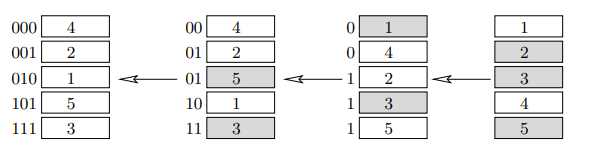
\includegraphics[scale=.5]{parada.png}
  \end{center}
  
%\pause
  
  \textbf{Obs.}:
  $\overline{\mathrm{Rif}} (\sigma) = {\mathrm{Rif}} (\sigma^{-1})$ e
  $\overline{U}(\sigma) = {U}(\sigma^{-1})$ logo
  $$\|{\rm Rif}^{(k)} - U\|_{\textsf{TV}} =
  \|\overline{\mathrm{Rif}}^{(k)} - \overline{U}\|_{\textsf{TV}}$$
\end{frame}


  
% ------------------------------------------------------------
\begin{frame}{A mistura por tempo de parada forte}
  
  Pelo lema anterior, a distância até a uniformidade após $k$
  embaralhamentos é $\le$ a probabilidade de \emph{ainda não
    termos parado}.
  
  
  \begin{block}{Corolário do Lema}
    Para todo $k \ge 0$,
    \[
      \| {\mathrm{Rif}}^{(k)} - U \|_{{\textsf{TV}}} \;\le\; \Pr(T >
      k).
    \]
  \end{block}
  
  %\pause
  
  
  \begin{block}{Leitura probabilística}
    \begin{itemize}
    \item Enquanto $ k < T $, \emph{ainda há dependência} entre as
      cartas.
    \item No instante $T$, \emph{o baralho está perfeitamente
        aleatório}.
    \item Assim, $\Pr(T > k)$ mede ``o quanto falta'' para atingir a
      uniformidade.
    \end{itemize}
  \end{block}
\end{frame}

% ------------------------------------------------------------
\begin{frame}{Tempo de parada  fortemente uniforme}


  \textbf{Para o \emph{riffle shuffle invertido}:}
  \[
    \Pr[T > k]
    = 1 - \prod_{i=1}^{n-1}\!\left(1 - \frac{i}{2^k}\right),
  \]
  análogo ao \emph{paradoxo do aniversário}: o embaralhamento
  ``mistura'' quando todos os rótulos binários das cartas se tornam
  distintos.

\end{frame}
  
% ------------------------------------------------------------
\begin{frame}[c]{Paradoxo do aniversário}
  
  Se $m$ pessoas nascem ao acaso em $m\ge n$ datas
  \[
    \begin{aligned}
      \Pr (\text{ não  colisão }) &=
      \frac{n(n-1)(n-2)\cdots(n-m+1)}{n^m} \\&=
      \left(1-\frac{1}{n}\right) \left(1-\frac{2}{n}\right)\cdots
      \left(1-\frac{m-2}{n}\right)
      \left(1-\frac{m-1}{n}\right)\\
      &\approx
      % \exp{\left(-\frac 1n\right)} \exp\left({-\frac 2n}\right) \cdots \exp\left(-\frac {m-1}n\right) \\ &=
      \exp \left( -\frac{m(m-1)}{2n} \right) \text{ para } m \lesssim
      \sqrt{n} 
    \end{aligned}
  \]

  pois
  
  $\displaystyle \prod_{i=1}^{m-1}(1-x_i) = \exp \left(
    \sum_{i=1}^{m-1} \ln(1-x_i) \right)$ e $\ln(1-x_i) \approx -x_i$
  para $x_i $ pequeno.
  
\end{frame}
% ------------------------------------------------------------
\begin{frame}{Interpretação via paradoxo do aniversário}

  \begin{itemize}
  \item O evento $[T \le k]$ equivale a \emph{``não há colisões de
      rótulos entre as $n$ cartas''}.
  
  \item 
    \(\displaystyle
      \Pr(\text{ não colisão }) = \prod_{i=1}^{n-1}\Big(1 -
      \frac{i}{2^k}\Big) \approx \exp\left(-\frac{n(n-1)}{2^{k+1}}
      \right)
    \)
  \item logo
\[
  \Pr[T>k] \approx 1 - \exp\Big(-\frac{n(n-1)}{2^{k+1}}\Big)
  \approx 1 - \exp\Big(-\frac{n^2}{2^{k+1}}\Big).
\]

Isto implica que a ausência de colisões (e, por consequência, a mistura em probabilidade/variação)
ocorre quando \(2^k \gg n^2\), i.e. para
\[
  k \approx 2\log_2 n + C, \quad C>0.
\]
    
\end{itemize}

\end{frame}

%------------------------------------------------------------
\begin{frame}{Exemplo numérico: baralho de 52 cartas}
  
  Para $n = 52$, a cota
  \[
    1 - \prod_{i=1}^{51}\Big(1 - \frac{i}{2^k}\Big)
  \]
  fornece limites superiores para a distância de variação total:
  
  \begin{center}
    \begin{tabular}{ccc}
      $k$ & $2^k$ & $1 - \prod(1 - i/2^k)$ \\ \hline
      6 & 64 & $\approx 1.00$ \\
      8 & 256 & $\approx 0.996$ \\
      10 & 1024 & $\approx 0.73$ \\
      11 & 2048 & $\approx 0.48$ \\
      12 & 4096 & $\approx 0.28$ \\
      13 & 8192 & $\approx 0.15$ \\
    \end{tabular}
  \end{center}
  
\end{frame}
% ------------------------------------------------------------


\end{document}
